\chapter{\texorpdfstring{MATHEMATICS}{}} %upper case only
\setcounter{equation}{0} \numberwithin{equation}{section}

\section{Small figures}
This section illustrates how to include a small .eps figure.
You can also use .pdf figures.
Run PDFLaTeX to compile the LaTeX source code.

\begin{figure}[h]
\centering
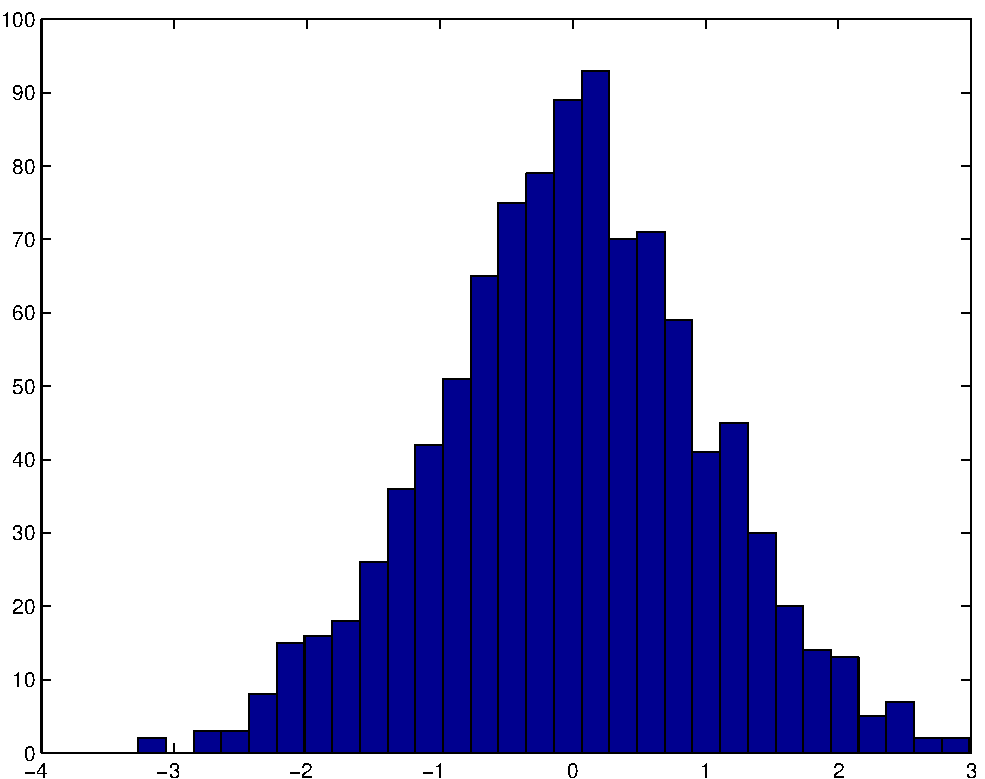
\includegraphics[width = 4.5 in ]{figures/figure-eps-converted-to.pdf}
\caption{Caption of a figure.}\label{FigureLabel}
\end{figure}

\section{Making tables}

\begin{table}[ht]
\centering \caption{The values of test
statistics and the corresponding critical values
at~$t_0.$~~$\alpha=0.1.$~}\label{stanford}\vskip .1in
\begin{tabular}{|c|c|c|c|c|c|c|}\hline
$t_0$ & 30 & 60 & 90 & 120 & 150 & 180 \\ \hline
Critical Value & 11.2282 & 10.5357 & 11.1108 & 11.7942 & 11.7343 & 11.7471\\ \hline
Test Statistic & 25.3182 & 24.6395 & 24.6049 & 25.6623 & 27.1320 & 29.3247\\ \hline
\end{tabular}
\end{table}

\section{Citations}

%If you use the package natbib for citations, here is the example how to cite an article.
%Many thanks to Dr. Maria Rizzo who worked this section.

To cite an article use cite, citet, or citep.

For ``in text'' citations use citet:  The original result is attributed to \citet{vn28}.
Refer to \citet{mardia70} for an example.
Refer to \cite{mardia70} for an example.

For a ``parenthetical citation'' use citep:  The computations were implemented in R \citep{R}
using bootstrap \citep{dh97,et93}.

When citing a book, it is helpful to mention where to find the result by indicating
a chapter or a page number or an equation number:  \citet[Ch.~6]{et93} discuss additional results.

Add your reference information to the file reference.bib.
Every time you edit reference.bib, run BibTeX on the dissertation.tex file so that LaTeX will know what the references are.

%If you don't want to use natbib, you should insert comment (\%) in the above part.  
%Here is the example to cite an article without using natbib package. \cite{forina1991class}

\section{Large, wide figures in landscape orientation}

It's not hard to incorporate very wide figures by making a landscape page in the middle of the PDF.  However, then you need the page number to move, in order to stay in the upper right corner.  That is handled by special LaTeX code in the following example.

\begin{landscape}
\thispagestyle{lscape}
\pagestyle{lscape}
  \begin{figure}
    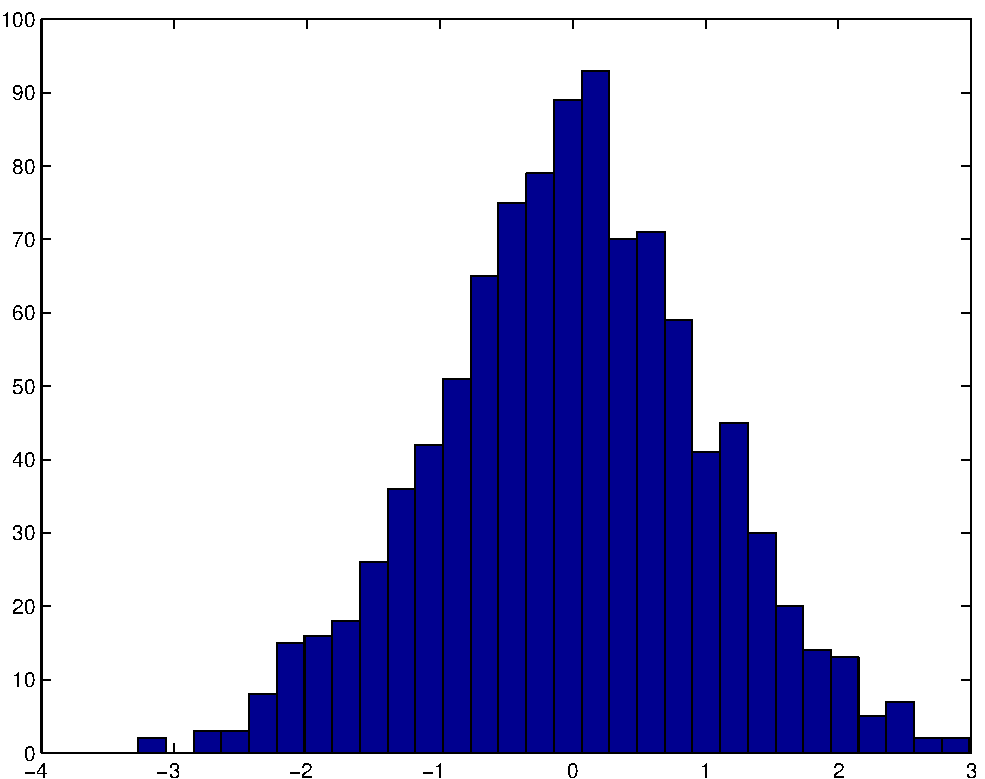
\includegraphics[width=\linewidth,height=\textheight-1in]{figures/figure.pdf}
    \caption[Short caption for List of Figures]{Long caption to appear under the figure.  Make sure the figure is small enough that the caption stays within the margins.  Note that the page number is still in the upper right corner of the PDF file; this is how it needs to be, so follow the code in chapter1.tex.}
  \end{figure}
\end{landscape}

\section{Definitions, Theorems, and proofs}
This section illustrates the normal appearance of definitions, theorems, proofs, and similar items in mathematical work.
Note that these are not listed in a separate list, unlike figures and tables.
All numbered items are counted using the same counter, including equations, theorems, lemmas, etc.
This is not a universal convention in mathematics, but it is super helpful for your readers to be able to find where a theorem or result is.
Also, since we can't have running headers indicating the chapter or section number, these numbers are helpful to indicate to the reader where they are in the document.

\begin{definition}
We say that $\lim_{x \to a} f(x) = L$ if for all $\varepsilon > 0$, there exists $\delta > 0$ such that for all $x \in (a-\delta,a+\delta),$ we have $|f(x) - L| < \varepsilon$.
\end{definition}

\begin{theorem}[Pythagorean Theorem]
For a right triangle with edge lengths $a$, $b$, and $c$ where $c$ is the length of the hypotenuse, 
\begin{equation}
    a^2 + b^2 = c^2
\end{equation}
\end{theorem}
\begin{proof}
Many proofs are available.  Here, we focus on the structure of the proof.

\noindent
{\bf Case 1:} Suppose that the triangle is isosceles.
Then $a = b$ and everything works out well.

\noindent
{\bf Case 2:} Suppose that the triangle is not isosceles.
The proof of this case is beyond the scope of this template.
\end{proof}

\section{Additional numbered results}

\begin{lemma}
A lemma is a short, technical result that is needed in the proof of a theorem.
\end{lemma}

Note how equations are numbered.
\begin{equation}
    (a+b)^2 = a^2 + 2 ab + b^2
\end{equation}

\begin{proposition}
A proposition is like a little theorem.
\end{proposition}

\begin{corollary}
A corollary is an easy result that follows a theorem.
\end{corollary}

